%%%%%%%%%%%%%%%%%%%%%%%%%%%%%%%%%%%%%%%%%%%%%%%%%%%%%%%%%%%%%%%%%%%%%%%%%%%%%%%%%%
\begin{frame}[fragile]\frametitle{}
\begin{center}
{\Large Yoganidra Course by Shrimath  -  Krishna Prakash}
\end{center}
\end{frame}

%%%%%%%%%%%%%%%%%%%%%%%%%%%%%%%%%%%%%%%%%%%%%%%%%%%%%%%%%%%%%%%%%%%%%%%%%%%%%%%%%%
\begin{frame}[fragile]\frametitle{}
\begin{center}
{\Large Day 1}
\end{center}
\end{frame}

%%%%%%%%%%%%%%%%%%%%%%%%%%%%%%%%%%%%%%%%%%%%%%%%%%%%%%%%%%%
\begin{frame}[fragile]\frametitle{Yoga Nidra  योगनिद्रा  -  A Tool for Self-Discovery}
      \begin{itemize}
        \item As per Swami Satyananda स्वामी सत्यानंद , Yoganidra is the first step towards transcendence (Samadhi समाधी )
		\item Yoganidra is mentioned in Yoga-Taravali योग तारावली  by Adi Shankara आदी शंकर 	  
        \item Helps navigate day-to-day challenges and seek the constant.
        \item Assists in self-inquiry - ``Who am I?'' and ``Why am I doing what I do?''.
        \item Bridges the material world (Mahamaya महामाया ) and pure consciousness.
        \item Supports achieving goals and ultimate self-realization, which is knowing who we are.
      \end{itemize}
\end{frame}

%%%%%%%%%%%%%%%%%%%%%%%%%%%%%%%%%%%%%%%%%%%%%%%%%%%%%%%%%%%
\begin{frame}[fragile]\frametitle{Aastika Darshana आस्तिक दर्शन  - The Knowledge Tradition}
      \begin{itemize}
        \item Aastika आस्तिक does not mean belief in God but belief in knowledge \& tradition.
        \item Knowledge (Veda वेद ) is born with creation.
        \item Veda is not a textbook but a body of knowledge passed through tradition.
        \item Pursuit of knowledge transcends caste, creed, and religion.
      \end{itemize}
\end{frame}

%%%%%%%%%%%%%%%%%%%%%%%%%%%%%%%%%%%%%%%%%%%%%%%%%%%%%%%%%%%
\begin{frame}[fragile]\frametitle{Trust in Tradition}
      \begin{itemize}
        \item When in doubt, trust the tradition of teachers, then
you are Aastika.
        \item A guide who has already experienced it can lead us beyond our intellect.
        \item Yoga Nidra belongs to the Aastika Darshana, derived from Tantra तंत्र , not classical Yoga.
      \end{itemize}
\end{frame}

%%%%%%%%%%%%%%%%%%%%%%%%%%%%%%%%%%%%%%%%%%%%%%%%%%%%%%%%%%%
\begin{frame}[fragile]\frametitle{Yoga Sutra योगसूत्र  \& Living Traditions}
      \begin{itemize}
        \item Yoga Sutra does not outline processes beyond meditation on OM.
        \item Processes are determined by the living traditions of the era.
        \item The goal is to reach the root of why one seeks Yoga Nidra.
      \end{itemize}
\end{frame}

%%%%%%%%%%%%%%%%%%%%%%%%%%%%%%%%%%%%%%%%%%%%%%%%%%%%%%%%%%%
\begin{frame}[fragile]\frametitle{Journey of Self-Discovery}
      \begin{itemize}
        \item ``Who am I?'' is a personal journey; no need for external validation.
        \item Understand yourself first; do not expect others to empathize.
        \item Doubts are welcome, but resolve them through understanding concepts.
      \end{itemize}
\end{frame}

%%%%%%%%%%%%%%%%%%%%%%%%%%%%%%%%%%%%%%%%%%%%%%%%%%%%%%%%%%%
\begin{frame}[fragile]\frametitle{Understanding Desire}
      \begin{itemize}
        \item Desire drives daily actions;  an emotion is energy in motion, similarly a thought that propels action is desire.
        \item Life is a series of desires - understanding them is crucial.
        \item Automated living leads to stress, insomnia, and rage.
        \item Exercise: Write a list of desires; do not share or judge them.
      \end{itemize}
\end{frame}

%%%%%%%%%%%%%%%%%%%%%%%%%%%%%%%%%%%%%%%%%%%%%%%%%%%%%%%%%%%
\begin{frame}[fragile]\frametitle{Tantra तंत्र - Channelizing Desires}
      \begin{itemize}
        \item Tantra provides methods to channel desires, not suppress them.
        \item Use Dharma धर्म  as a filter to refine desires.
        \item Infinite desires exist but can be classified into four categories (Purushartha पुरुषार्थ).
      \end{itemize}
\end{frame}

%%%%%%%%%%%%%%%%%%%%%%%%%%%%%%%%%%%%%%%%%%%%%%%%%%%%%%%%%%%
\begin{frame}[fragile]\frametitle{Purushartha - The Four Desires}
Buckets for ideas, desires , goals:
      \begin{itemize}
        \item Dharma धर्म : Role clarity, duties, righteousness, understanding right or wrong.
        \item Artha अर्थ : Wealth generation, using intellect for decisions. This appreciates with time. You use mind to take this type of decision. Need to generate wealth
for the other three categories (bramacharya ब्रह्मचर्य , vanaprastha वानप्रस्थ , sanyasa सन्यास). Getting fooled to think if
you are spiritual you should be poor these are all pedal ideas don't believe that. Health is probably wealth (wellness because of it appreciates with time)
        \item Kaama काम :  Sense pleasures, using body \& senses for decisions. This depreciates with time.
        \item Moksha मोक्ष : Ultimate self-realization, the common goal. We can keep it aside as one common desire out of infinite desires. So all remaining desires can now be classified into remaining 3 categories. That's the authority of Indian Traditions.
        \item Rule: Artha \& Kaama are valid if aligned with Dharma.
      \end{itemize}
\end{frame}

%%%%%%%%%%%%%%%%%%%%%%%%%%%%%%%%%%%%%%%%%%%%%%%%%%%%%%%%%%%
\begin{frame}[fragile]\frametitle{Antahkarana अंत : करण - The Inner Instrument}

Where does the thinking/processing is happening?: Antahkarana अंत : करण (inner instrument, 'M'ind), works in 4 different modes:
      \begin{itemize}
        \item Manas मनस (Mind): Collects thoughts, generates desires.
        \item Buddhi बुद्धी (Intellect): Decision making, applying filters.
        \item Chitta चित्त (Memory): Storage of past experiences.
        \item Ahamkara अहंकार (Ego): Self-identity, action initiator. Self Arrogating Principle, helps us take action. Inferiority \& superiority complexes stem from a sense of lack. 
        \item Ego should be used mindfully to implement what is intellectually right.
        \item Willpower plays a key role in executing our decisions.
        \item Balance between intellect and action is necessary for growth.
      \end{itemize}
\end{frame}

%%%%%%%%%%%%%%%%%%%%%%%%%%%%%%%%%%%%%%%%%%%%%%%%%%%%%%%%%%%
\begin{frame}[fragile]\frametitle{Processes for Inner Clarity}
      \begin{itemize}
        \item Yoga Nidra योगनिद्रा : Calms the mind and aids goal realization.
        \item Antarmouna अंतरमौन : Inner silence practice for self-reflection.
        \item Bhramari Pranayama भ्रामरी प्राणायाम : Breathing technique for calming the mind.
        \item Mantra Sadhana मंत्र साधना : Chanting practice to enhance focus and awareness.
      \end{itemize}
\end{frame}

% %%%%%%%%%%%%%%%%%%%%%%%%%%%%%%%%%%%%%%%%%%%%%%%%%%%%%%%%%%%%%%%%%%%%%%%%%%%%%%%%%%
% \begin{frame}[fragile]\frametitle{}
% \begin{center}
% {\Large Desires List}
% \end{center}
% \end{frame}

% %%%%%%%%%%%%%%%%%%%%%%%%%%%%%%%%%%%%%%%%%%%%%%%%%%%%%%%%%%%
% \begin{frame}[fragile]\frametitle{Desires List Classification}
      % \begin{itemize}
        % \item In the Indian tradition, one first fulfills duties (Dharma धर्म ), then generates resources (Artha अर्थ ), and finally enjoys pleasures (Kāma काम ), all in service of Mokṣa मोक्ष .
        % \item Artha and Kāma are only approved when they serve Dharma.
		% \item Anything to do with you as a individual comes under Dharma anything Clarity you need as a person comes under Dharma.
      % \end{itemize}
% \end{frame}

% %%%%%%%%%%%%%%%%%%%%%%%%%%%%%%%%%%%%%%%%%%%%%%%%%%%%%%%%%%%
% \begin{frame}[fragile]\frametitle{Family \& Social Desires}
      % \begin{itemize}
        % \item \textbf{Better education, life for kids} - Providing quality education is a duty. \textbf{(Artha)}
        % \item \textbf{Better fulfilling career for wife} - Supporting spouse’s career is ethical and beneficial. \textbf{(Artha)}
        % \item \textbf{Good Health for Parents} - Caring for parents is a dharmic duty. \textbf{(Dharma)}
        % \item \textbf{Global respect, popularity, recognition on social media} - Elevates status, builds influence. \textbf{(Artha)}
      % \end{itemize}
% \end{frame}

% %%%%%%%%%%%%%%%%%%%%%%%%%%%%%%%%%%%%%%%%%%%%%%%%%%%%%%%%%%%
% \begin{frame}[fragile]\frametitle{Health \& Well-Being Desires}
% Desires which are purely personal in nature which helps you build to do further actions, like Health, come under Dharma, ie Deh-Dharma देहधर्म 
      % \begin{itemize}
        % \item \textbf{Chronic fatigue/tiredness to go} - Restoring energy to fulfill duties. \textbf{(Dharma)}
        % \item \textbf{7–8 hrs of sound, deep sleep} - Essential for mental clarity and health. \textbf{(Dharma)}
        % \item \textbf{Migraine headache to go} - Needed for focus and efficiency. \textbf{(Dharma)}
        % \item \textbf{Less cholesterol} - Optimizing health for long-term productivity. \textbf{(Dharma)}
        % \item \textbf{Big arms} - Pursuit of aesthetics and physical pride. \textbf{(Kāma)}
        % \item \textbf{Flat abs} - Focused on body appearance and social admiration. \textbf{(Kāma)}
      % \end{itemize}
% \end{frame}

% %%%%%%%%%%%%%%%%%%%%%%%%%%%%%%%%%%%%%%%%%%%%%%%%%%%%%%%%%%%
% \begin{frame}[fragile]\frametitle{Summary of Desires Classification}
      % \begin{itemize}
        % \item \textbf{Dharma (Duty \& Righteous Living)}
        % \begin{itemize}
          % \item Primary health goals: Ending chronic fatigue, achieving deep sleep, eliminating migraines
          % \item Health optimization: Less cholesterol
          % \item Good Health for parents
        % \end{itemize}
        % \item \textbf{Artha (Wealth, Health, and Resource Building)}
        % \begin{itemize}
          % \item Better education, life for kids
          % \item Better fulfilling career for wife		
          % \item Global respect, popularity, recognition on social media
        % \end{itemize}
        % \item \textbf{Kāma (Sense Pleasures \& Aesthetic Desires)}
        % \begin{itemize}
          % \item Bodily aesthetics: Big arms, flat abs
        % \end{itemize}
      % \end{itemize}
	  
	  % A generic desire could be: I want Good Intellect, Good Strength and Calm Mind. चांगली बुद्धी, शक्ती, शांत स्वरूप दे
% \end{frame}

%%%%%%%%%%%%%%%%%%%%%%%%%%%%%%%%%%%%%%%%%%%%%%%%%%%%%%%%%%%%%%%%%%%%%%%%%%%%%%%%%%
\begin{frame}[fragile]\frametitle{}
\begin{center}
{\Large Day 2}
\end{center}
\end{frame}


%%%%%%%%%%%%%%%%%%%%%%%%%%%%%%%%%%%%%%%%%%%%%%%%%%%%%%%%%%%
\begin{frame}[fragile]\frametitle{Paper and Magnifying Glass Analogy}
      \begin{itemize}
      \item Paper is our mind and Magnifying Glass is our body.
      \item Holding glass steady: Sun-rays converge—\textbf{Pratyāhāra} (\textbf{प्रत्याहार}, Withdrawal).
      \item Keeping body \& mind still: Black circle forms—\textbf{Dhāraṇā} (\textbf{धारणा}, Concentration).
      \item Spark appears—\textbf{Dhyāna} (\textbf{ध्यान}, Meditation).
      \item Paper burns—\textbf{Samādhi} (\textbf{समाधि}, Transcendence).
      \end{itemize}
\end{frame}

%%%%%%%%%%%%%%%%%%%%%%%%%%%%%%%%%%%%%%%%%%%%%%%%%%%%%%%%%%%
\begin{frame}[fragile]\frametitle{Types of Yoganidra}
      \begin{itemize}
      \item Common Yoganidra is of \textbf{Pratyāhāra} type.
      \item There are also \textbf{Dhāraṇā} and \textbf{Dhyāna} Yoganidra.
      \item Awareness ≠ Attention-Focus-Concentration (\textbf{Dhāraṇā}).
      \item In Pratyāhāra-Yoganidra, we must \textbf{be aware}, not concentrate.
      \item Yoganidra: \textbf{Ears open, Eyes closed}.
      \end{itemize}
\end{frame}

%%%%%%%%%%%%%%%%%%%%%%%%%%%%%%%%%%%%%%%%%%%%%%%%%%%%%%%%%%%
\begin{frame}[fragile]\frametitle{Inner Journey: Vector, Not Scalar}
      \begin{itemize}
      \item Inner journey is \textbf{Vector} (Direction matters more than speed).
      \item Scalar movement (just going) doesn't help.
      \item Speed \& Direction both define true inner progress.
      \end{itemize}
\end{frame}

%%%%%%%%%%%%%%%%%%%%%%%%%%%%%%%%%%%%%%%%%%%%%%%%%%%%%%%%%%%
\begin{frame}[fragile]\frametitle{Importance of Sound in Yogic Tradition}
      \begin{itemize}
      \item Sound is the subtlest sensory input.
      \item Ears capture sound, not eyes.
      \item 60-80% of knowledge comes via vision—eyes dominate senses.
      \item Visual takes more energy, sound requires more attention \& retention.
      \item \textbf{Vedas are \textit{Shrutis} (श्रुति)}—heard, not written.
      \end{itemize}
\end{frame}

%%%%%%%%%%%%%%%%%%%%%%%%%%%%%%%%%%%%%%%%%%%%%%%%%%%%%%%%%%%
\begin{frame}[fragile]\frametitle{Levels of Yoganidra Practice}
      \begin{itemize}
      \item \textbf{Level 1}: Awareness circulation (joints), body relaxation.
      \item \textbf{Level 2}: Awareness of spaces between joints + breath (\textbf{Prāṇamaya Kośa} \textbf{प्राणमय कोश}).
      \item \textbf{Brain’s “Little Man”} has a body map—triggered during awareness rotation.
      \item Body relaxation (\textbf{Annamaya Kośa} \textbf{अन्नमय कोश}) is a must.
      \end{itemize}
\end{frame}

%%%%%%%%%%%%%%%%%%%%%%%%%%%%%%%%%%%%%%%%%%%%%%%%%%%%%%%%%%%
\begin{frame}[fragile]\frametitle{Preparatory Stages for Yoganidra}
      \begin{itemize}
      \item \textbf{Prāṇāyāma} (\textbf{प्राणायाम}): \textbf{Bhrāmarī} (\textbf{भ्रामरी}).
      \item \textbf{Antar Mauna} (\textbf{अंतर मौन}) - Inner Silence.
      \item \textbf{Mantra Sādhanā} (\textbf{मन्त्र साधना}) - Mantra Discipline.
      \item These enhance readiness for deeper \textbf{Yoganidra}.
      \end{itemize}
\end{frame}

%%%%%%%%%%%%%%%%%%%%%%%%%%%%%%%%%%%%%%%%%%%%%%%%%%%%%%%%%%%
\begin{frame}[fragile]\frametitle{Sense Profile: Understanding Yourself}
      \begin{itemize}
      \item Mind is an \textbf{aggregate of senses}.
      \item \textbf{Sense Mastery} > Mind Mastery.
      \item Without Sense Mastery, Mind Mastery is unstable.
      \item \textbf{Pratyāhāra} focuses on sense mastery—gateway to inner yoga.
      \end{itemize}
\end{frame}

%%%%%%%%%%%%%%%%%%%%%%%%%%%%%%%%%%%%%%%%%%%%%%%%%%%%%%%%%%%
\begin{frame}[fragile]\frametitle{Sense Profile Matrix (5x3)}
      \begin{itemize}
      \item 5 Senses: \textbf{Sound (Shabda \textbf{शब्द}), Touch (Sparsha \textbf{स्पर्श}), Form (Rūpa \textbf{रूप}), Taste (Rasa \textbf{रस}), Smell (Gandha \textbf{गंध})}.
      \item Profile: \textbf{Like (L), Neutral (N), Dislike (D)}.
      \item Example: Like cotton texture, neutral to linen, dislike polyester.
      \end{itemize}
\end{frame}

%%%%%%%%%%%%%%%%%%%%%%%%%%%%%%%%%%%%%%%%%%%%%%%%%%%%%%%%%%%
\begin{frame}[fragile]\frametitle{Being a Witness in Antar Mouna \& Yoganidra}
      \begin{itemize}
      \item Identify sense triggers in meditation.
      \item Simply \textbf{witness} the reaction, mentally note, move on.
      \item Stay \textbf{present}—maximize effort in the now.
      \end{itemize}
\end{frame}

%%%%%%%%%%%%%%%%%%%%%%%%%%%%%%%%%%%%%%%%%%%%%%%%%%%%%%%%%%%
\begin{frame}[fragile]\frametitle{Main Tenet: “What Can I Do Now?”}
      \begin{itemize}
      \item Irritating sound? Witness it.
      \item If action possible—act (e.g., oiling a creaky door).
      \item Otherwise—\textbf{accept and remain silent}.
      \end{itemize}
\end{frame}

%%%%%%%%%%%%%%%%%%%%%%%%%%%%%%%%%%%%%%%%%%%%%%%%%%%%%%%%%%%
\begin{frame}[fragile]\frametitle{Benefits of Yoganidra}
      \begin{itemize}
      \item Develop skill to \textbf{respond, not react}.
      \item Shift from \textbf{Sympathetic Nervous System} (Fight or Flight) to \textbf{Parasympathetic} (Relax \& Digest).
      \item Recognize difference between \textbf{getting anger} vs. \textbf{showing anger}.
      \item Cultivate \textbf{dexterity in response}.
      \end{itemize}
\end{frame}

% %%%%%%%%%%%%%%%%%%%%%%%%%%%%%%%%%%%%%%%%%%%%%%%%%%%%%%%%%%%%%%%%%%%%%%%%%%%%%%%%%%
% \begin{frame}[fragile]\frametitle{}
% \begin{center}
% {\Large Senses Profile}
% \end{center}
% \end{frame}

% %%%%%%%%%%%%%%%%%%%%%%%%%%%%%%%%%%%%%%%%%%%%%%%%%%%%%%%%%%%
% \begin{frame}[fragile]\frametitle{Sense Profile}
      % \begin{itemize}
          % \item In Indic thought, senses (\textit{indriyas} \textbf{इन्द्रिय}) are not just for perception but also sources of affect (attraction or aversion).
          % \item Sensory experiences can be categorized into three: Like, Neutral, and Dislike.
      % \end{itemize}
% \end{frame}

% %%%%%%%%%%%%%%%%%%%%%%%%%%%%%%%%%%%%%%%%%%%%%%%%%%%%%%%%%%%
% \begin{frame}[fragile]\frametitle{Sound (shabda शब्द ) Hearing (\textit{Śravaṇa} \textbf{श्रवण})}
      % \begin{itemize}
          % \item \textbf{Like:} Soothing classical \textit{rāga} \textbf{राग} or gentle sound of flowing river.
          % \item \textbf{Neutral:} Soft murmur of ambient noise—distant chatter or rustling leaves.
          % \item \textbf{Dislike:} Harsh, discordant sounds—screeching alarm or nails on chalkboard.
      % \end{itemize}
% \end{frame}

% %%%%%%%%%%%%%%%%%%%%%%%%%%%%%%%%%%%%%%%%%%%%%%%%%%%%%%%%%%%
% \begin{frame}[fragile]\frametitle{Touch (\textit{Sparśa} \textbf{स्पर्श})}
      % \begin{itemize}
          % \item \textbf{Like:} Comforting feel of silk or gentle caress.
          % \item \textbf{Neutral:} Ordinary texture of everyday cotton fabric—neither pleasant nor unpleasant.
          % \item \textbf{Dislike:} Rough, abrasive surface—coarse sandpaper or uncomfortably cold surface.
      % \end{itemize}
	  
% Relative to 3 things, Triputi त्रिपुटी:  Situation, Object, People.
% \end{frame}

% %%%%%%%%%%%%%%%%%%%%%%%%%%%%%%%%%%%%%%%%%%%%%%%%%%%%%%%%%%%
% \begin{frame}[fragile]\frametitle{Form (roop रूप ) Sight (\textit{Darśana} \textbf{दर्शन})}
      % \begin{itemize}
          % \item \textbf{Like:} Awe-inspiring view of a vibrant sunrise or blooming lotus.
          % \item \textbf{Neutral:} Observing a plain, unadorned wall—neither exciting nor disturbing.
          % \item \textbf{Dislike:} Chaotic, jarring display—garish or distorted image causing discomfort.
      % \end{itemize}
% \end{frame}


% %%%%%%%%%%%%%%%%%%%%%%%%%%%%%%%%%%%%%%%%%%%%%%%%%%%%%%%%%%%
% \begin{frame}[fragile]\frametitle{Taste (\textit{Rasa} \textbf{रस})}
      % \begin{itemize}
          % \item \textbf{Like:} Delightful sweetness of ripe mango or honey.
          % \item \textbf{Neutral:} Bland taste—plain water or unsalted rice.
          % \item \textbf{Dislike:} Overly bitter or sour flavor—unpalatable herbal decoction or spoiled food.
      % \end{itemize}
% \end{frame}



% %%%%%%%%%%%%%%%%%%%%%%%%%%%%%%%%%%%%%%%%%%%%%%%%%%%%%%%%%%%
% \begin{frame}[fragile]\frametitle{Smell (gandh गंध ) (\textit{Ghrāṇa} \textbf{घ्राण})}
      % \begin{itemize}
          % \item \textbf{Like:} Uplifting aroma of jasmine or sandalwood.
          % \item \textbf{Neutral:} Faint scent of fresh air or clean linen—does not strongly affect mood.
          % \item \textbf{Dislike:} Repulsive odor—rotting food or decay.
      % \end{itemize}
% \end{frame}



% %%%%%%%%%%%%%%%%%%%%%%%%%%%%%%%%%%%%%%%%%%%%%%%%%%%%%%%%%%%
% \begin{frame}[fragile]\frametitle{Conclusion}
      % \begin{itemize}
          % \item Sensory experiences shape perception and emotional response.
          % \item Understanding attraction, neutrality, and aversion helps in mindful engagement with the world.
      % \end{itemize}
% \end{frame}


%%%%%%%%%%%%%%%%%%%%%%%%%%%%%%%%%%%%%%%%%%%%%%%%%%%%%%%%%%%%%%%%%%%%%%%%%%%%%%%%%%
\begin{frame}[fragile]\frametitle{}
\begin{center}
{\Large Day 3}
\end{center}
\end{frame}

%%%%%%%%%%%%%%%%%%%%%%%%%%%%%%%%%%%%%%%%%%%%%%%%%%%%%%%%%%%
\begin{frame}[fragile]\frametitle{Nonlinear Traditional Systems}
      \begin{itemize}
          \item Modern education is linear, whereas traditional systems are nonlinear.
          \item Nonlinear approach helps thrive in chaos.
          \item Indian leadership excels due to exposure to nonlinear learning (60s-70s generation).
          \item Complete adoption of the Western linear model may lead to losing this advantage.
      \end{itemize}
\end{frame}

%%%%%%%%%%%%%%%%%%%%%%%%%%%%%%%%%%%%%%%%%%%%%%%%%%%%%%%%%%%
\begin{frame}[fragile]\frametitle{Holistic Perspective on Life}
      \begin{itemize}
          \item Life is cyclical, not linear.
          \item Existence is eternal; आत्मा (Atman) never dies.
          \item A holistic approach shapes reactions and responses.
          \item Reaction can sometimes be the best response.
          \item Balancing sympathetic and parasympathetic nervous systems enhances well-being.
      \end{itemize}
\end{frame}

%%%%%%%%%%%%%%%%%%%%%%%%%%%%%%%%%%%%%%%%%%%%%%%%%%%%%%%%%%%
\begin{frame}[fragile]\frametitle{$\delta$ Delta Waves - Deep Sleep \& Healing}
      \begin{itemize}
          \item Essential for deep sleep, cellular repair, and regeneration.
          \item Lack of delta sleep accelerates aging and cognitive decline.
          \item Caregivers must prioritize deep sleep for well-being.
          \item Improvement strategies:
            \begin{itemize}
                \item Practice योग निद्रा (Yoga Nidra) before bedtime.
                \item Maintain a consistent sleep routine.
                \item Perform Shavasana शवासन (Corpse Pose) for deep relaxation.
            \end{itemize}
      \end{itemize}
\end{frame}

%%%%%%%%%%%%%%%%%%%%%%%%%%%%%%%%%%%%%%%%%%%%%%%%%%%%%%%%%%%
\begin{frame}[fragile]\frametitle{$\beta$ Beta Waves - Alertness \& Decision Making}
      \begin{itemize}
          \item Beta waves support decision-making and mental alertness.
          \item Excessive beta activity leads to anxiety and gut issues.
          \item Overanalyzing and debating excessively increase beta waves.
          \item Beta waves may be linked to the \textbf{Vagus Nerve} in future research.
          \item Improvement strategies:
            \begin{itemize}
                \item Practice सूर्य नमस्कार (Surya Namaskar) to improve focus.
                \item Perform मंत्र साधना (Mantra Sadhana) to stabilize beta waves.
                \item Engage in puzzles or learn new skills to balance cognition.
            \end{itemize}
      \end{itemize}
\end{frame}

%%%%%%%%%%%%%%%%%%%%%%%%%%%%%%%%%%%%%%%%%%%%%%%%%%%%%%%%%%%
\begin{frame}[fragile]\frametitle{$\gamma$ Gamma Waves - Learning \& Concentration}
      \begin{itemize}
          \item Gamma waves enhance deep focus and cognitive function.
          \item Passion and hobbies naturally stimulate gamma waves.
          \item योग (Yoga) suggests भ्रामरी (Bhramari) for gamma wave activation.
          \item Perform भ्रामरी (Bhramari) for 6.5 to 7 minutes in one sitting.
          \item Improvement strategies:
            \begin{itemize}
                \item Practice भ्रामरी (Bhramari) to enhance gamma wave production.
                \item Perform dynamic योग आसन (Yoga Asanas) for mental stimulation.
                \item Cultivate or restart hobbies for cognitive engagement.
            \end{itemize}
      \end{itemize}
\end{frame}

%%%%%%%%%%%%%%%%%%%%%%%%%%%%%%%%%%%%%%%%%%%%%%%%%%%%%%%%%%%
\begin{frame}[fragile]\frametitle{$\theta$ Theta Waves - Creativity \& Intuition}
      \begin{itemize}
          \item Theta waves enhance creativity, memory, and emotional balance.
          \item ब्रह्म मुहूर्त (Brahma Muhurta) - optimal time for study, meditation.
          \item संध्या उपासना (Sandhya Upasana) aligns with theta wave transitions (sunrise, sunset, noon).
          \item Theta waves increase with surrender, trust, and deep conversations.
          \item Improvement strategies:
            \begin{itemize}
                \item Practice योग निद्रा (Yoga Nidra) to deepen theta activity.
                \item Engage in creative visualizations and activities.
                \item Chant sacred texts (श्री विष्णु / श्री ललिता सहस्रनाम, कुरान, श्री गुरु ग्रंथ साहिब, बाइबिल) for 20 minutes daily.
            \end{itemize}
      \end{itemize}
\end{frame}

%%%%%%%%%%%%%%%%%%%%%%%%%%%%%%%%%%%%%%%%%%%%%%%%%%%%%%%%%%%
\begin{frame}[fragile]\frametitle{$\alpha$ Alpha Waves - Relaxation \& Mindfulness}
      \begin{itemize}
          \item Alpha state is cultivated through consistent inner work.
          \item Cannot be instantly generated through weekend programs.
          \item Indic wisdom simplifies overwhelming thoughts into structured categories.
          \item Being present in the now aids evolution and maturity.
          \item Developing a witness attitude naturally shifts one into alpha state.
          \item Mindful work and love for the process enhance alpha waves.
          \item Face problems with a calm mind: "What can I do now?"
          \item Improvement strategies:
            \begin{itemize}
                \item Practice योग निद्रा (Yoga Nidra) to enhance relaxation.
                \item Perform नाड़ी शोधन (Nadi Shodhana) to calm the mind.
                \item Spend time in nature or listen to soothing music.
            \end{itemize}
      \end{itemize}
\end{frame}

%%%%%%%%%%%%%%%%%%%%%%%%%%%%%%%%%%%%%%%%%%%%%%%%%%%%%%%%%%%
\begin{frame}[fragile]\frametitle{Role of मनस् (Manas) in Brain Waves}
      \begin{itemize}
          \item मनस् (Manas) governs brain wave generation and mental processes.
          \item Overthinking and intellectualizing can be turned into strengths.
          \item Anchor the mind through regular साधना (Sadhana).
          \item Despite life’s challenges, meditation should continue.
          \item मंत्र (Mantra) leads to silence; sound is the soundest of साधना (Sadhanas).
          \item Mantra, प्राणायाम (Pranayama), and hobbies provide stability.
      \end{itemize}
\end{frame}

%%%%%%%%%%%%%%%%%%%%%%%%%%%%%%%%%%%%%%%%%%%%%%%%%%%%%%%%%%%
\begin{frame}[fragile]\frametitle{Mantra Practice - The Path to Silence}
      \begin{itemize}
          \item जप (Japa) is conscious repetition of sound for the advised duration.
          \item Mind wanders for 10 seconds; train it to withdraw.
          \item Let the mind go; hold on to the mantra like a boat on a lake.
          \item Swami Satyananda स्वामी सत्यानंद : Do not force concentration; just be with the mantra with love.
          \item Despite life’s uncertainties, mantra practice shifts the mindset positively.
          \item Mindfulness in mantra ensures there is no past, future, or present—only the now.
          \item Three stages of mantra practice:
            \begin{itemize}
                \item \textbf{ जप (Loud Japa)}: Helps correct pronunciation and calms the beta state.
                \item \textbf{उपांशु (Upamshu)}: Whispered mantra, audible only to oneself.
                \item \textbf{मानसिक (Manasika)}: Silent internal repetition, absorbed into the spiritual heart.
            \end{itemize}
      \end{itemize}
\end{frame}

%%%%%%%%%%%%%%%%%%%%%%%%%%%%%%%%%%%%%%%%%%%%%%%%%%%%%%%%%%%%%%%%%%%%%%%%%%%%%%%%%%
\begin{frame}[fragile]\frametitle{}
\begin{center}
{\Large Day 4}
\end{center}
\end{frame}

%%%%%%%%%%%%%%%%%%%%%%%%%%%%%%%%%%%%%%%%%%%%%%%%%%%%%%%%%%%
\begin{frame}[fragile]\frametitle{Regular Practice and Mind Tricks}
      \begin{itemize}
        \item Without practice, the mind constantly seeks more knowledge.
        \item With regular practice, a shift happens naturally.
        \item Reduce usage of words like 'feel', 'like', 'dislike' to improve life.
        \item Mind tricks us; fixed practice times like sunrise, sunset, or noon help.
        \item \textbf{Dinacharya (दिनचर्या ) and Rutucharya (ऋतुचर्या )} are crucial.
      \end{itemize}
\end{frame}

%%%%%%%%%%%%%%%%%%%%%%%%%%%%%%%%%%%%%%%%%%%%%%%%%%%%%%%%%%%
\begin{frame}[fragile]\frametitle{Consistency in Practice}
      \begin{itemize}
        \item Skipping practice for 3 days can derail progress.
        \item Fourth day becomes difficult to return to practice.
        \item Inner journey is unlike an office job; think like an entrepreneur.
        \item Certifications fail as people treat yoga like a degree.
        \item Practice is like daily habits—brushing, eating, etc.
        \item \textbf{Nitya Karma Anushthan (नित्य कर्म अनुष्ठान)} is essential.
      \end{itemize}
\end{frame}

%%%%%%%%%%%%%%%%%%%%%%%%%%%%%%%%%%%%%%%%%%%%%%%%%%%%%%%%%%%
\begin{frame}[fragile]\frametitle{Depth vs Breadth in Practice}
      \begin{itemize}
        \item Depth is more important than breadth in the inner journey.
        \item Knowledge comes from breadth, but revelations come from depth.
        \item Repetition is key to insights.
        \item Tradition emphasizes repeating the same process for thousands of years.
        \item Example: \textbf{Gayatri Mantra (गायत्री मंत्र)} practice over generations.
      \end{itemize}
\end{frame}

%%%%%%%%%%%%%%%%%%%%%%%%%%%%%%%%%%%%%%%%%%%%%%%%%%%%%%%%%%%
\begin{frame}[fragile]\frametitle{Mantra: The Vehicle to Silence}
      \begin{itemize}
        \item Mantra leads to inner silence.
        \item Two approaches: \textbf{Naam Mantra (नाम मंत्र)}, \textbf{Beej Mantra (बीज मंत्र)}.
        \item \textbf{Beej Mantra} needs initiation (e.g., 'Om' ॐ ).
        \item \textbf{Naam Mantra} (e.g., 'Namah Shivay' नमः शिवाय) is more accessible.
        \item Teacher selects mantra based on student's capacity.
      \end{itemize}
\end{frame}

%%%%%%%%%%%%%%%%%%%%%%%%%%%%%%%%%%%%%%%%%%%%%%%%%%%%%%%%%%%
\begin{frame}[fragile]\frametitle{Sharing and Growth in Practice}
      \begin{itemize}
        \item Indian classical music requires training, but anyone can hum a song.
        \item Initiation requires a teacher, but we are all fellow seekers.
        \item True sharing means sharing what is given, like passing a lit lamp.
        \item The more you share, the more you grow.
      \end{itemize}
\end{frame}

%%%%%%%%%%%%%%%%%%%%%%%%%%%%%%%%%%%%%%%%%%%%%%%%%%%%%%%%%%%
\begin{frame}[fragile]\frametitle{Essence of Ancient Texts}
      \begin{itemize}
        \item First verse gives the essence of ancient texts.
        \item \textbf{Yogasutra: योगसूत्र } 'Atha Yoganushasanam (अथ योगानुशासनम्)' - Study of 'Now'.
        \item Objective: Establish us in the present through discipline.
        \item Explains pitfalls, siddhis सिद्धी, and methods to develop concentration.
      \end{itemize}
\end{frame}

%%%%%%%%%%%%%%%%%%%%%%%%%%%%%%%%%%%%%%%%%%%%%%%%%%%%%%%%%%%
\begin{frame}[fragile]\frametitle{Bhagavad Gita and Dharma}
      \begin{itemize}
        \item \textbf{Bhagavad Gita: भगवद्गीता } Begins with 'Dharmakshetre (धर्मक्षेत्रे)'.
        \item Entire text explains \textbf{Dharma (धर्म)} and duties via Yoga योग  (Karma कर्म , Bhakti भक्ती , Raja राज ).
        \item Shastras शास्त्र are called \textbf{Darshanas (दर्शन)} as they provide vision.
      \end{itemize}
\end{frame}

%%%%%%%%%%%%%%%%%%%%%%%%%%%%%%%%%%%%%%%%%%%%%%%%%%%%%%%%%%%
\begin{frame}[fragile]\frametitle{Lalita Sahasranama ललित सहस्त्रनाम : The Divine Mother}
      \begin{itemize}
        \item Describes the divine mother \textbf{Shri Mata (श्री माता)}.
        \item She is the source of all—creator, preserver, and destroyer.
        \item Invocation varies: Durga दुर्गा for obstacles, Lakshmi लक्ष्मी for wealth, Saraswati सरस्वती for wisdom.
        \item Whatever is needed in life comes from her.
      \end{itemize}
\end{frame}

%%%%%%%%%%%%%%%%%%%%%%%%%%%%%%%%%%%%%%%%%%%%%%%%%%%%%%%%%%%
\begin{frame}[fragile]\frametitle{Yoga Nidra and Creativity}
      \begin{itemize}
        \item Yoga Nidra योगनिद्रा helps realize personal resolutions.
        \item Life constantly pushes us to be creative and innovative.
        \item Being in touch with creation leads to better problem-solving.
        \item \textbf{Mantra for this session: 'Om Shree Matre Namah (ॐ श्री मात्रे नमः)'}.
      \end{itemize}
\end{frame}

%%%%%%%%%%%%%%%%%%%%%%%%%%%%%%%%%%%%%%%%%%%%%%%%%%%%%%%%%%%
\begin{frame}[fragile]\frametitle{Mantra Sadhana मंत्र साधना : Inner Purification}
      \begin{itemize}
        \item 80-90\% of Indians practice sadhana to acquire things.
        \item In traditional practice, mantra sadhana मंत्र साधना  focuses on:
        \item \textbf{Chitta Shuddhi (चित्त शुद्धि)} - Purification of mind.
        \item \textbf{Chitta Ekagrata (चित्त एकाग्रता)} - Concentration.
        \item \textbf{Chitta Vishalata (चित्त विशालता)} - Expansiveness.
        \item Inner work aligns us with the larger system of existence.
      \end{itemize}
\end{frame}



%%%%%%%%%%%%%%%%%%%%%%%%%%%%%%%%%%%%%%%%%%%%%%%%%%%%%%%%%%%%%%%%%%%%%%%%%%%%%%%%%%
\begin{frame}[fragile]\frametitle{}
\begin{center}
{\Large Day 5}
\end{center}
\end{frame}


%%%%%%%%%%%%%%%%%%%%%%%%%%%%%%%%%%%%%%%%%%%%%%%%%%%%%%%%%%%%%%%%%%%%%%%%%%%%%%%%%%
\begin{frame}[fragile]\frametitle{}
	\begin{center}
	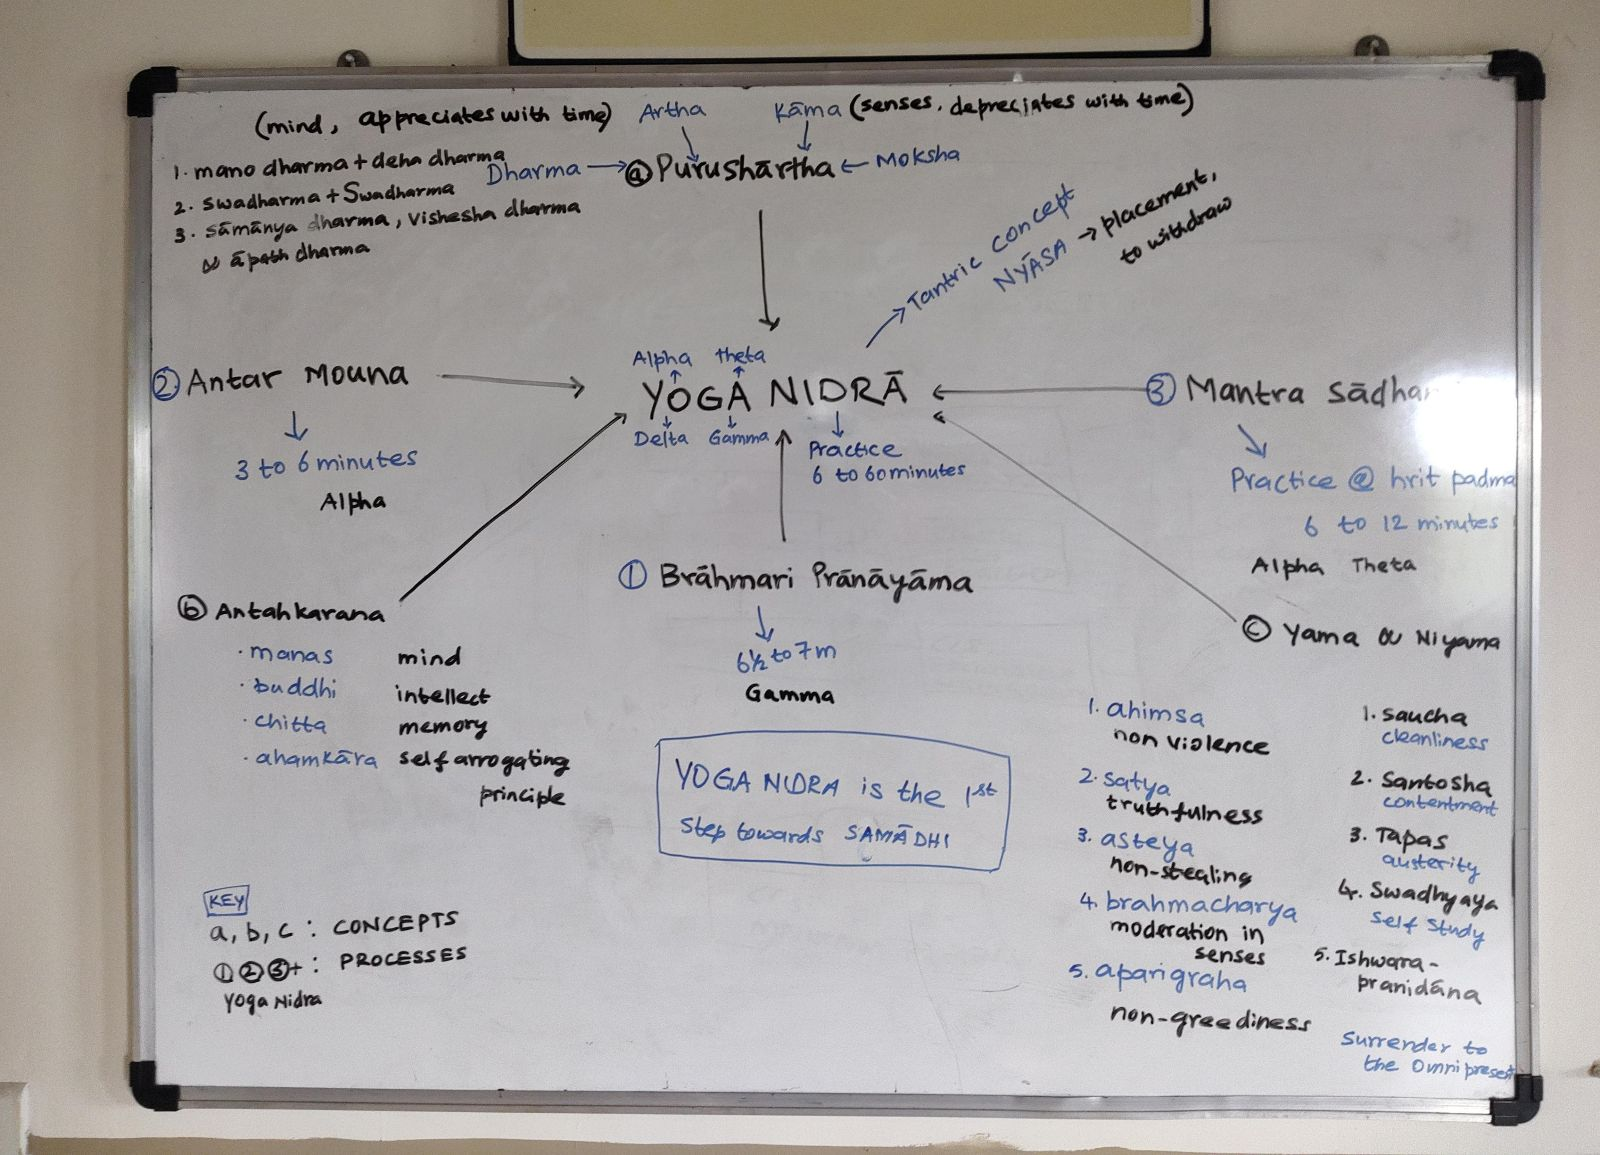
\includegraphics[width=\linewidth,keepaspectratio]{Shrimath_Yoganidra_Mindmap}
	\end{center}	
\end{frame}

%%%%%%%%%%%%%%%%%%%%%%%%%%%%%%%%%%%%%%%%%%%%%%%%%%%%%%%%%%%
\begin{frame}[fragile]\frametitle{Awareness and Waves}
      \begin{itemize}
        \item Awareness is like standing on a seashore.
        \item Waves (thoughts, sounds) come on their own.
        \item No effort is needed to chase them.
        \item In youth, we rush towards experiences.
        \item Maturity: Stand still, waves reach you naturally.
        \item Awareness happens on its own—just be present.
      \end{itemize}
\end{frame}

%%%%%%%%%%%%%%%%%%%%%%%%%%%%%%%%%%%%%%%%%%%%%%%%%%%%%%%%%%%
\begin{frame}[fragile]\frametitle{Yoga Nidra and Nyasa (न्यास)}
      \begin{itemize}
        \item Yoga Nidra originates from \textbf{Nyasa (न्यास)}.
        \item \textbf{Nyasa} (Tantra) = Tried and tested method.
        \item Two meanings: Placement and Withdrawal.
        \item \textbf{Sannyasa (संन्यास)} = Samyak + Nyasa (Perfect withdrawal).
        \item Withdrawing from personal identity; world is family.
        \item Awareness of instructions, no distractions.
      \end{itemize}
\end{frame}

%%%%%%%%%%%%%%%%%%%%%%%%%%%%%%%%%%%%%%%%%%%%%%%%%%%%%%%%%%%
\begin{frame}[fragile]\frametitle{Yoga Nidra and Brain Waves}
      \begin{itemize}
        \item Yoga Nidra balances Alpha and Theta waves.
        \item State: Neither fully asleep nor awake.
        \item Detached witness to distractions.
        \item Enables relaxation, healing, and stress reduction.
        \item Reduces blood pressure and anxiety.
      \end{itemize}
\end{frame}

%%%%%%%%%%%%%%%%%%%%%%%%%%%%%%%%%%%%%%%%%%%%%%%%%%%%%%%%%%%
\begin{frame}[fragile]\frametitle{Mantra (मन्त्र) - The Anchor}
      \begin{itemize}
        \item \textbf{Mantra (मन्त्र)} = Mananat Trayate Iti (मननात् त्रायते इति).
        \item Acts as an anchor in changing life circumstances.
        \item Mood, age, problems change—mantra remains constant.
        \item Regular practice enhances self-healing and mindfulness.
      \end{itemize}
\end{frame}

%%%%%%%%%%%%%%%%%%%%%%%%%%%%%%%%%%%%%%%%%%%%%%%%%%%%%%%%%%%
\begin{frame}[fragile]\frametitle{Dharma (धर्म) - Support and Stability}
      \begin{itemize}
        \item \textbf{Dharma (धर्म)} = That which sustains and supports.
        \item Balance between goal pursuit and emotional resilience.
        \item \textbf{Mano Dharma (मनो धर्म)} = Duty towards the mind.
        \item \textbf{Deha Dharma (देह धर्म)} = Duty towards the body.
        \item Ask: Is my goal aligned with \textbf{Swadharma (स्वधर्म)}?
      \end{itemize}
\end{frame}

%%%%%%%%%%%%%%%%%%%%%%%%%%%%%%%%%%%%%%%%%%%%%%%%%%%%%%%%%%%
\begin{frame}[fragile]\frametitle{Swadharma (स्वधर्म) and Passion}
      \begin{itemize}
        \item Swadharma (self-duty) aligns passion and profession.
        \item If aligned, less marketing needed—service attracts people.
        \item Misalignment = More strategy, planning, and effort.
        \item Example: A hockey player playing cricket for money.
      \end{itemize}
\end{frame}

%%%%%%%%%%%%%%%%%%%%%%%%%%%%%%%%%%%%%%%%%%%%%%%%%%%%%%%%%%%
\begin{frame}[fragile]\frametitle{Yama (यम) and Niyama (नियम)}
      \begin{itemize}
        \item Foundations of Yoga: Yama (यम) and Niyama (नियम).
        \item Useful for refining resolves and desires.
        \item Guides personal discipline and ethical conduct.
      \end{itemize}
\end{frame}

%%%%%%%%%%%%%%%%%%%%%%%%%%%%%%%%%%%%%%%%%%%%%%%%%%%%%%%%%%%
\begin{frame}[fragile]\frametitle{Sankalpa (संकल्प) vs Affirmation}
      \begin{itemize}
        \item Affirmations: Passive, mind-centered, unreliable.
        \item Sankalpa (संकल्प): Active, action-based self-discovery.
        \item Self-chosen—not decided by others.
        \item Rooted in present reality, not abstract desires.
      \end{itemize}
\end{frame}

%%%%%%%%%%%%%%%%%%%%%%%%%%%%%%%%%%%%%%%%%%%%%%%%%%%%%%%%%%%
\begin{frame}[fragile]\frametitle{Framing a Sankalpa (संकल्प)}
      \begin{itemize}
        \item Must be a \textbf{Need}, not just a Want.
        \item Avoid over-ambitious or abstract resolutions.
        \item Focus on what disturbs the mind most.
        \item Resolve must be personal—not for others.
        \item Specific, measurable, and positively framed.
        \item Example: “I need optimum sound sleep.”
      \end{itemize}
\end{frame}

%%%%%%%%%%%%%%%%%%%%%%%%%%%%%%%%%%%%%%%%%%%%%%%%%%%%%%%%%%%
\begin{frame}[fragile]\frametitle{Yoga Nidra - Practical Tips}
      \begin{itemize}
        \item Avoid stiffness—Corpse pose, but not a corpse.
        \item Be still but respond to discomfort (e.g., mosquito).
        \item Use a light blanket—Body temperature may drop.
      \end{itemize}
\end{frame}

%%%%%%%%%%%%%%%%%%%%%%%%%%%%%%%%%%%%%%%%%%%%%%%%%%%%%%%%%%%
\begin{frame}[fragile]\frametitle{Process of Yoga Nidra}
      \begin{itemize}
        \item \textbf{Bhramari (भ्रामरी)} - 7 minutes
        \item \textbf{Antar Mouna (अंतर मौन)} - 2-3 minutes
        \item \textbf{Yoga Nidra (योगनिद्रा)} - 25-35 minutes
        \item \textbf{Mantra Sadhana (मन्त्र साधना)} - 5 minutes
      \end{itemize}
\end{frame}

%%%%%%%%%%%%%%%%%%%%%%%%%%%%%%%%%%%%%%%%%%%%%%%%%%%%%%%%%%%
\begin{frame}[fragile]\frametitle{Levels of Yoga Nidra}
      \begin{itemize}
        \item Level 1: Awareness rotation at joints. (annamaya kosha अन्नमय कोष )
        \item Level 2: Awareness rotation between joints. (annamaya kosha अन्नमय कोष )
        \item Level 3: Awareness rotation + Breath-work. (pranamaya kosha प्राणमय कोष )
        \item Level 4: Awareness rotation + Breath-work + Resolve + Visualizations. (manomaya kosha मनोमय कोष )
      \end{itemize}
\end{frame}


%%%%%%%%%%%%%%%%%%%%%%%%%%%%%%%%%%%%%%%%%%%%%%%%%%%%%%%%%%%%%%%%%%%%%%%%%%%%%%%%%%
\begin{frame}[fragile]\frametitle{}
\begin{center}
{\Large What is Really Yoga Nidra -  Krishna Prakash}

{\tiny (Ref: Practising the Art of Deep Rest: A Conversation on Yoga Nidra \& Mental Stillness - The Art of Zen Living)}
\end{center}
\end{frame}

%%%%%%%%%%%%%%%%%%%%%%%%%%%%%%%%%%%%%%%%%%%%%%%%%%%%%%%%%%%
\begin{frame}[fragile]\frametitle{What is Yoga Nidra?}
      \begin{itemize}
	\item Nidra means sleep; Yoga Nidra is conscious sleep
	\item Aware while mimicking sleep - connecting with that which never sleeps
	\item First step to transcendence in traditional yoga
	\item Helps transcend limitations like stress and anxiety
	\item Different from regular sleep - maintains awareness throughout
	\item Traditional tool for inner transformation and self-realization
	\item Connects us with our true nature beyond mental fluctuations
	  \end{itemize}
\end{frame}

%%%%%%%%%%%%%%%%%%%%%%%%%%%%%%%%%%%%%%%%%%%%%%%%%%%%%%%%%%%
\begin{frame}[fragile]\frametitle{Mind-Body Connection}
      \begin{itemize}
	\item Body is hardware, mind is software, prana is electricity
	\item What manifests in mind first affects the body
	\item Fear creates shivering, sweat, and irregular breathing
	\item Ancient wisdom recorded these connections in Yoga Sutras
	\item Stress manifests as physical depression and dejection
	\item Software (mind) changes reflect in hardware (body)
	\item Knowledge is ancient, only terminology is modern
	  \end{itemize}
\end{frame}

%%%%%%%%%%%%%%%%%%%%%%%%%%%%%%%%%%%%%%%%%%%%%%%%%%%%%%%%%%%
\begin{frame}[fragile]\frametitle{Deep Relaxation vs Regular Relaxation}
      \begin{itemize}
	\item Regular relaxation: shopping, entertainment, sense gratifications
	\item Deep relaxation: understanding impermanence of all things
	\item External achievements are temporary and relative
	\item Success today may become obsolete tomorrow
	\item Mind-level preparation needed before using techniques
	\item Conceptual understanding of letting go is essential
	\item Yoga Nidra enables cellular repair through delta waves
	\item No judgment if you sleep during practice
	  \end{itemize}
\end{frame}

%%%%%%%%%%%%%%%%%%%%%%%%%%%%%%%%%%%%%%%%%%%%%%%%%%%%%%%%%%%
\begin{frame}[fragile]\frametitle{The Five Brain Waves}
      \begin{itemize}
	\item Alpha: Present moment awareness, no judgment, meditation state
	\item Beta: Transactional activities, discussions, can lead to burnout
	\item Gamma: High concentration, deep focus, enhanced cognition
	\item Theta: Healing state, early morning consciousness, enhanced memory
	\item Delta: Deep relaxation, cellular repair, natural during yoga nidra
	\item Each wave serves specific purposes when balanced
	\item Understanding waves helps identify personal imbalances
	  \end{itemize}
\end{frame}

%%%%%%%%%%%%%%%%%%%%%%%%%%%%%%%%%%%%%%%%%%%%%%%%%%%%%%%%%%%
\begin{frame}[fragile]\frametitle{Hustle Culture and Sleep}
      \begin{itemize}
	\item Any culture without rest, relaxation, sleep should be avoided
	\item Short-term gains meaningless if health is compromised
	\item Must be alive and healthy to enjoy achievements
	\item Trends come and go, traditional wisdom remains constant
	\item Sleep deprivation affects brain functioning significantly
	\item Goals and desires often prevent proper sleep
	\item Mind culture more important than external cultures
	  \end{itemize}
\end{frame}

%%%%%%%%%%%%%%%%%%%%%%%%%%%%%%%%%%%%%%%%%%%%%%%%%%%%%%%%%%%
\begin{frame}[fragile]\frametitle{Filtering Desires Through Dharma}
      \begin{itemize}
	\item Write down all desires without suppression or judgment
	\item Don't share personal desires - they are uniquely yours
	\item Use dharma as a filter for your aspirations
	\item Many sleepless nights caused by unprocessed to-do lists
	\item Written desires have better chances of fulfillment
	\item Plant desires as seeds in yoga nidra practice
	\item Understand your unique body-mind constitution (Ayurveda)
	\item Distinguish your goals from others' expectations
	  \end{itemize}
\end{frame}

%%%%%%%%%%%%%%%%%%%%%%%%%%%%%%%%%%%%%%%%%%%%%%%%%%%%%%%%%%%
\begin{frame}[fragile]\frametitle{Yoga Nidra vs Hypnosis}
      \begin{itemize}
	\item Hypnosis: Remote control with therapist/psychologist
	\item Yoga Nidra: You maintain control throughout practice
	\item Only you know what prevents your sleep
	\item Self-empowerment rather than external dependence
	\item Structured process from relaxation to self-understanding
	\item Knowledge creates curiosity for deeper practice
	\item Learn from traditional sources for proper understanding
	\item Work is needed - no magic wand solutions
	  \end{itemize}
\end{frame}

%%%%%%%%%%%%%%%%%%%%%%%%%%%%%%%%%%%%%%%%%%%%%%%%%%%%%%%%%%%
\begin{frame}[fragile]\frametitle{Benefits of Yoga Nidra Practice}
      \begin{itemize}
	\item Enables delta wave production naturally
	\item Promotes cellular level repair and healing
	\item Improves cognitive function and mental clarity
	\item Helps sync with natural circadian rhythms
	\item Provides deep rest without external cost
	\item Develops witness consciousness and non-judgment
	\item Supports transcendence of personal limitations
	\item Creates foundation for spiritual growth
	  \end{itemize}
\end{frame}

%%%%%%%%%%%%%%%%%%%%%%%%%%%%%%%%%%%%%%%%%%%%%%%%%%%%%%%%%%%
\begin{frame}[fragile]\frametitle{Essential Practice Guidelines}
      \begin{itemize}
	\item Maintain erect spine with relaxed shoulders
	\item Keep eyes closed, breathe only through nostrils
	\item Begin as witness to surrounding sounds
	\item Progress to witnessing breath without controlling it
	\item Visualize a comfortable, peaceful place mentally
	\item Pray for good health with self-compassion
	\item Return awareness gradually to present moment
	\item End with palm warmth on eyelids before opening eyes
	  \end{itemize}
\end{frame}

%%%%%%%%%%%%%%%%%%%%%%%%%%%%%%%%%%%%%%%%%%%%%%%%%%%%%%%%%%%
\begin{frame}[fragile]\frametitle{Key Wisdom from Tradition}
      \begin{itemize}
	\item "If you protect dharma, dharma protects you"
	\item Every day is good - unfavorable circumstances aid inner growth
	\item "Even this will pass away" - perspective on impermanence
	\item Every place is peaceful - disturbance comes from within
	\item No magic solutions - consistent practice and work required
	\item Learn from traditional sources with authentic lineage
	\item Knowledge is eternal, expressions change with time
	\item Mind deserves equal attention as body
	  \end{itemize}
\end{frame}